%%%%%%%%%%%%%%%%%%%%%%%%%%%%%%%%%%%%%%%%%%%%%%%%%%%%%%%%%%%%%%%%%%%%%%%%%%%%%%
%                 Chapter 4
%
%%%%%%%%%%%%%%%%%%%%%%%%%%%%%%%%%%%%%%%%%%%%%%%%%%%%%%%%%%%%%%%%%%%%%%%%%%%%%%
\chapter{Risultati numerici}
\label{cap:cp4}

In questa sezione riportiamo alcuni test effettuati sia con il metodo
MCM che con MCM \emph{volume preserving}. Il programma che fa girare
questi due schemi è stato realizzato in \emph{C programming language},
per il cui sorgente \cite[vedi][]{vpmcm:code}. Inizieremo col testare
il programma su superfici standard lisce tipo sfera,toro e manubrio; e
poi aggiungeremo alcuni tipi di rumore ripulendo le superfici con i
due metodi evidenziandone le differenze. Infine testeremo entrambi su
un immagine reale sia in presenza che in assenza di rumore.

%%%%%%%%%%%%%%%%%%%%%%%%%%%%%%%%%%%%%%%%%%%%%%%%%%%%%%%%%%%%%%%%%%%%%%%%%%%%%%
%                 Section 4.1
%
%%%%%%%%%%%%%%%%%%%%%%%%%%%%%%%%%%%%%%%%%%%%%%%%%%%%%%%%%%%%%%%%%%%%%%%%%%%%%%
\section{Test su superfici standard}
\label{sec:cp4-sc1}
Iniziamo col far evolvere una sfera, quindi prendiamo il seguente dato
iniziale

\[
u_0(x) = \max\left(r_0^2-|x|^2,0\right)
\]


\begin{wrapfloat}{figure}{l}{0pt}
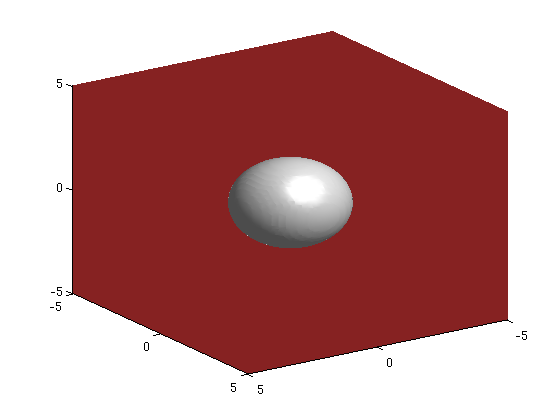
\includegraphics[scale=0.50,width=0.5\textwidth]{smooth/vpmcm/sphere/sphere0}
\caption{Sfera al tempo $t=0$, relaticva al livello $5.0$}
\end{wrapfloat}

dove abbiamo scelto $r_0=3$ e il livello $5.0$, quindi il nostro dato
iniziale sarà una sfera di raggio $2$. Facendola evolvere usando il  metodo
MCM (vedi \emph{Fig}\ref{fig:cp4-sc1-01}), come abbiamo anticipato
in §\ref{sec:cp1-sc2}, la sfera perde sempre di più il suo volume, in
quanto il raggio dimnuisce sempre di più, finchè non si annulla ad un
tempo finito (tempo di collasso) riducendo la sfera ad un semplice punto. Mentre
con il metodo MCM \emph{volume presetving}, il termine di trasporto
riesce a bilanciare la perdita di volume, mantenendo la sfera pressochè
costante;come si può notare dalla \emph{Tab}\ref{tab:cp4-sc1-01}
 l'errore tra il volume iniziale e quello finale, si riduce
 all'aumentare del numero dei nodi, cioè $\Delta x\to 0$.

\begin{osservazione}[Approssimazione del volume]
Il volume delle superfici, ad un dato livello,  sia al tempo iniziale
che finale è stato apprssimato utilizzando la formula del punto medio
in $\mathbb{R}^3$ sul seguente integrale
\[
\int_{\Omega\subseteq\mathbb{R}^3}(1-H(u(x)))dx
\]
dove $H(u(x))$ è la funzione di Heaviside definita in \eqref{eq:cp3-sc3-1-add-01}.
\end{osservazione}

\begin{table}[htb!]
\caption{Tabella per lo schema PVMCM. Evoluzione di una sfera nel cubo $[-4,4]^3$.}
\label{tab:cp4-sc1-01}
\[
\begin{array}{*{5}{c}l}
    \toprule
    \text{time} &\text{nodi} &\Delta t &\text{iter} &\text{CPUs}&\text{VolErr} \\
    \midrule
     0.05       & 50         & 0.16    & 1          & 0,4s      &7.2e^{-01}\\ 
 %               &            & 0.04    & 3          & 1,3s      &1.4e^{-01}\\
     0.2        &            &         & 2          & 0.8s      &1.3\\
 %               &            & 0.04    & 3          & 1.3s      &3.5e^{-01}\\
     0.4        &            &         & 3          & 1,3s      &2.2\\ 
 %               &            & 0.04    & 10         & 6,1s      &9.4e^{-01}\\
     0.8        &            &         & 5          & 2.4s      &4.4\\
     \midrule
     0.05       & 100        & 0.08    & 1          & 3,0s      &3.8e^{-02}\\ 
     0.2        &            &         & 3          & 9.4s      &1.2e^{-01}\\
     0.4        &            &         & 5          & 16,9s     &1.9e^{-01}\\ 
     0.8        &            &         & 10         & 39s       &6.7e^{-02}\\
    \bottomrule
\end{array}
\]
\end{table}

\begin{figure}[htb!]
  \centering
  \subfloat[][\emph{MCM: Sfera al tempo} $t=0.2$.]
           {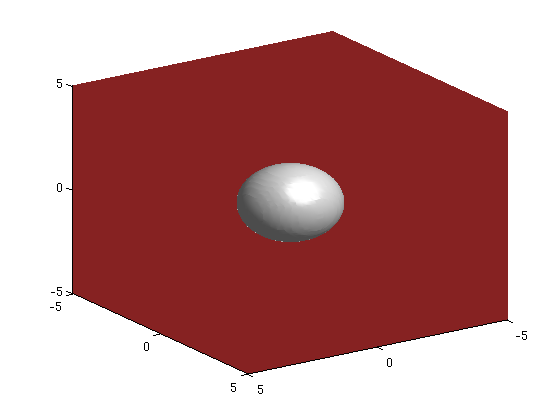
\includegraphics[width=.45\textwidth]{smooth/mcm/sphere/sphere50-2-02}}\quad
  \subfloat[][\emph{MCM: Sfera al tempo} $t=0.8$.]
           {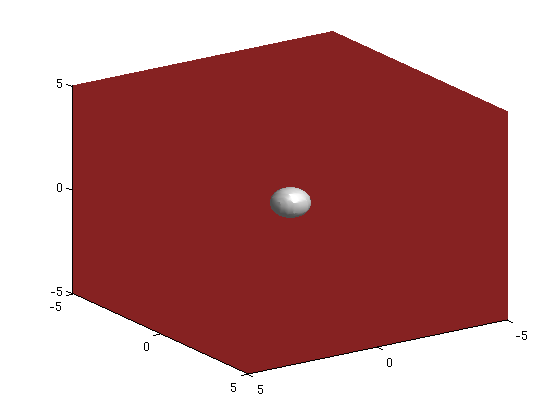
\includegraphics[width=.45\textwidth]{smooth/mcm/sphere/sphere50-4-08}}\\
  \subfloat[][\emph{PVMCM: Sfera al tempo} $t=0.2$.]
           {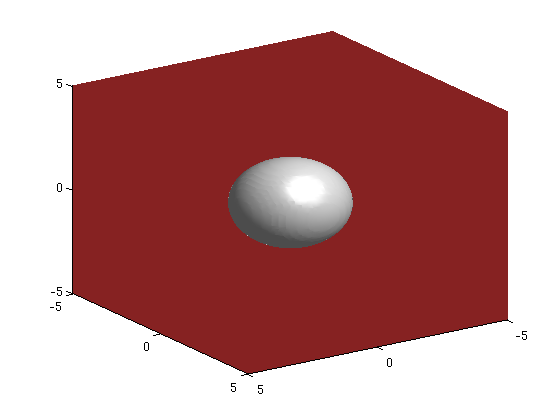
\includegraphics[width=.45\textwidth]{smooth/vpmcm/sphere/sphere2}}\quad
  \subfloat[][\emph{PVMCM: Sfera al tempo} $t=0.8$.]
           {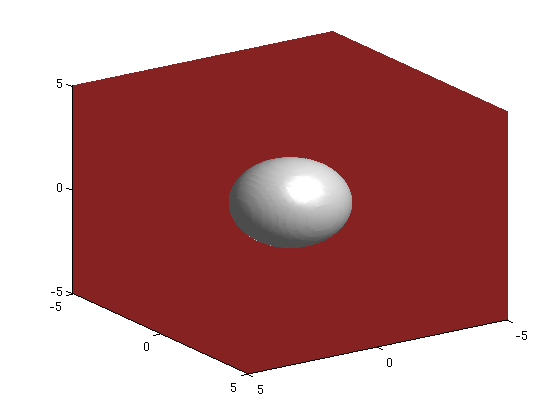
\includegraphics[width=.45\textwidth]{smooth/vpmcm/sphere/sphere4}}\quad
  \caption{Evoluzione della Sfera}
  \label{fig:cp4-sc1-01}
\end{figure}

\newpage
Passiamo ora ad un'altra famosa superfice, il toro. La funzione
level-set del toro è data da
\[
u_0(x) = \left(R_0-\sqrt{x^2+y^2}\right)+z^2-r_0^2.
\]

\begin{wrapfloat}{figure}{l}{0pt}
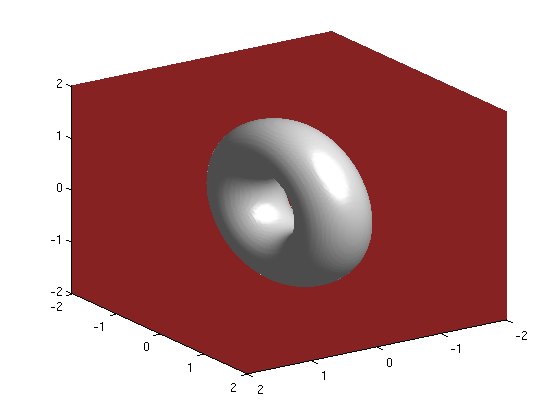
\includegraphics[scale=0.50,width=0.5\textwidth]{smooth/vpmcm/torus/torus100-0-00}
\caption{Toro al tempo $t=0$, relativ al livello $0$}
\end{wrapfloat}

Dove abbiamo preso $R_0=1.0$, $r_0=0.5$ e insieme di livello zero. Lo
schema MCM (vedi \emph{Fig.} ), fa pian piano collassare il toro ad
una circonferenza, in quanto $r_0$ diminuisce più rapidamente di
$R_0$.  Mentre il volume preserving cerca di conservare il volume
iniziale  allungando la superfice del toro come si vede in
\emph{Fig}\ref{fig:cp4-sc1-02}. Un comportamento diverso si ha se
prendiamo $R_0<r_0$, in tal caso MCM mi fa convergere il toro ad una
sfera, che poi questa a sua volta collasserà in un punto; mentre il
volume preserving si comporta nello stesso modo. Anche qui riportiamo
gli errori del volume preserving nella \emph{Tab}\ref{tab:cp4-sc1-02}.

\begin{figure}[htb!]
  \centering
  \subfloat[][\emph{MCM: Toro al tempo} $t=0.05$.]
           {\includegraphics[width=.45\textwidth]{smooth/mcm/torus/torus100-2-005}}\quad
  \subfloat[][\emph{MCM: Toro al tempo} $t=0.12$.]
           {\includegraphics[width=.45\textwidth]{smooth/mcm/torus/torus100-4-012}}\\
  \subfloat[][\emph{PVMCM: Toro al tempo} $t=0.05$.]
           {\includegraphics[width=.45\textwidth]{smooth/vpmcm/torus/torus100-2-005}}\quad
  \subfloat[][\emph{PVMCM: Toro al tempo} $t=0.12$.]
           {\includegraphics[width=.45\textwidth]{smooth/vpmcm/torus/torus100-4-012}}\quad
  \caption{Evoluzione del Toro}
  \label{fig:cp4-sc1-02}
\end{figure}

\begin{table}[htb!]
\caption{Tabella per lo schema PVMCM. Evoluzione del Toro nel cubo $[-2,2]^3$.}
\label{tab:cp4-sc1-02}
\[
\begin{array}{*{5}{c}l}
    \toprule
    \text{time} &\text{nodi} &\Delta t &\text{iter} &\text{CPUs}&\text{VolErr} \\
    \midrule
     0.03       & 100        & 0.04    & 1          & 13s      &1.8e^{-01}\\
     0.05       &            &         & 2          & 26s      &4.6e^{-01}\\ 
     0.09       &            &         & 3          & 38,7s    &9.5e^{-01}\\ 
     0.12       &            &         & 3          & 38.7s    &9,5e^{-01}\\
     \midrule
     0.03       & 200        & 0.02    & 2          & 207s     &8.2e^{-02}\\ 
     0.05       &            &         & 3          & 310s     &1.4e^{-01}\\
     0.09       &            &         & 5          & 514s     &3.6e^{-01}\\ 
     0.12       &            &         & 6          & 618s     &4.5e^{-01}\\
    \bottomrule
\end{array}
\]
\end{table}

\newpage

Terminiamo questa mini sezione, presentando i risultati ottenuti
facendo evolvere una superfice non convessa, \emph{il manubrio}.

\begin{wrapfloat}{figure}{l}{0pt}
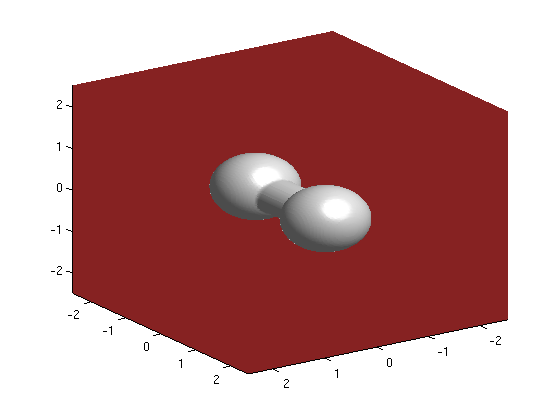
\includegraphics[scale=0.50,width=0.5\textwidth]{smooth/vpmcm/dumbbell/dumbb100-0-00}
\caption{Manubrio al tempo $t=0$, relativ al livello $0.1$}
\end{wrapfloat}

Tale superficie è ottenuta prendendo il massimo tra due sfere di raggo
$R_0=0.8$ ed un cilindro di raggio $r_0=0.5$, il tutto calcolato al
livello $0.1$. Come osservato in §\ref{sec:cp1-sc2}, l'evoluzione di
superfici non convesse secondo il moto per curvatura media può
generare delle singolarità. Difatti applicando lo schema MCM, il
cilindro tende rapidamente a collassare in una linea mentre le due
sfere continuano ad evolversi in altre sfere self-similar. Finchè il
manubrio si divide in due sfere disconnesse, a questo puto è cambiata
la topologia della superfice iniziale e le due sfere collassano
separatamente in un punto (vedi \emph{Fig}\ref{fig:cp4-sc1-03}).
Mentre il volume preserving, contrasta il collasso rapido  del
cilindro allungando il manubrio e riesce ad ritardare il cambiamento
topologico vedi \emph{Fig}\ref{fig:cp4-sc1-03}. Riportiamo in \emph{Tab}\ref{tab:cp4-sc1-03}  gli errori
della conservazione del volume.

\begin{table}[htb!]
\caption{Tabella per lo schema PVMCM. Evoluzione del Manubrio nel cubo $[-2,2]^3$}
\label{tab:cp4-sc1-03}
\[
\begin{array}{*{5}{c}l}
    \toprule
    \text{time} &\text{nodi} &\Delta t &\text{iter} &\text{CPUs}&\text{VolErr} \\
    \midrule
     0.04       & 100        & 0.005   & 8          & 11.5s    &6.1e^{-02}\\
     0.06       &            &         & 12         & 19s      &1.1e^{-01}\\ 
     0.08       &            &         & 16         & 29s      &1.5e^{-01}\\ 
     0.09       &            &         & 18         & 34s      &1,9e^{-01}\\
     0.1        &            &         & 20         & 39s      &2.5e^{-01}\\     
     \bottomrule
\end{array}
\]
\end{table}

\begin{figure}[htb!]
  \centering
  \subfloat[][\emph{MCM: Manubrio al tempo} $t=0.06$.]
           {\includegraphics[width=.45\textwidth]{smooth/mcm/dumbbell/dumbb100-2-006}}\quad
  \subfloat[][\emph{MCM: Manubrio al tempo} $t=0.1$.]
           {\includegraphics[width=.45\textwidth]{smooth/mcm/dumbbell/dumbb100-5-01}}\\
  \subfloat[][\emph{PVMCM: Manubrio al tempo} $t=0.06$.]
           {\includegraphics[width=.45\textwidth]{smooth/vpmcm/dumbbell/dumbb100-2-006}}\quad
  \subfloat[][\emph{PVMCM: Manubrio al tempo} $t=0.1$.]
           {\includegraphics[width=.45\textwidth]{smooth/vpmcm/dumbbell/dumbb100-5-01}}\quad
  \caption{Evoluzione del Manubrio}
  \label{fig:cp4-sc1-03}
\end{figure}

%%%%%%%%%%%%%%%%%%%%%%%%%%%%%%%%%%%%%%%%%%%%%%%%%%%%%%%%%%%%%%%%%%%%%%%%%%%%%%
%                 Section 4.2
%
%%%%%%%%%%%%%%%%%%%%%%%%%%%%%%%%%%%%%%%%%%%%%%%%%%%%%%%%%%%%%%%%%%%%%%%%%%%%%%
\section{\emph{Denoising} su superfici standard}

In questa sezione vediamo come i due metodi si comportano nel
\emph{denoising}, cioè nel togliere il rumore dalle immagini. Iniziamo
prima a ripulire le superfi standard, di cui prima abbiamo parlato,
per poi passare ad immagini 3D reali. Per aggiungere il rumore
utilizzeremo sia una funzione random che la funzione \emph{imnoise} di
MATLAB, che aggiunge un rumore \emph{gaussiano}. Quest'ultima aggiunge
più o meno rumore a seconda dei valori di media e varianza che
inseriamo, quelli di default sono $0$ ed $0.1$. Mentre la funzione
random genera un numero random di sfere, da noi inserito, con i centri
in punti random appartenenti all'intervallo in considerazione e i
raggi random scelti in un range da zero ad un numero da noi
inserito. Ogni volta che un punto della griglia cade in una di queste
sfere, aggiungiamo un valore random ad $u_0(x)$ scelto in un range tra
zero ed un valore da noi inserito.

%%%%%%%%%%%%%%%%%%%%%%%%%%%%%%%%%%%%%%%%%%%%%%%%%%%%%%%%%%%%%%%%%%%%%%%%%%%%%%
%                 Section 4.2.1
%
%%%%%%%%%%%%%%%%%%%%%%%%%%%%%%%%%%%%%%%%%%%%%%%%%%%%%%%%%%%%%%%%%%%%%%%%%%%%%%
\subsection{\emph{Random Noise}}
Iniziamo col analizzare il caso della sfera. Questa è stata prima
sporcata con la funzione random e poi è stata fatta evolvere con
entrambi i metodi.
I dati iniziali della sfera solo identici a quelli nella sezione
precedente, mentre il volume iniziale è stato calcolato includendo
anche il rumore.

\begin{wrapfloat}{figure}{l}{0pt}
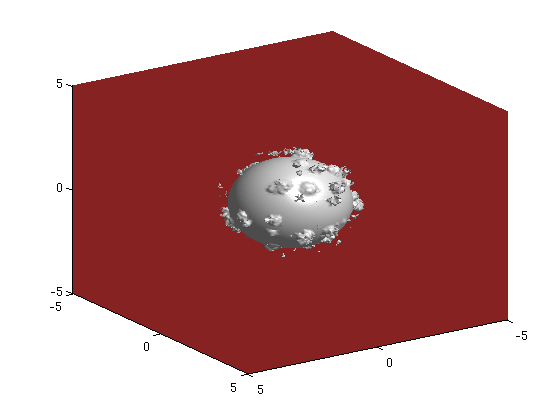
\includegraphics[scale=0.50,width=0.5\textwidth]{noise/randNoise/vpmcm/sphere/sphere100r-0-00}
\caption{Sfera al tempo $t=0$, sporcata con rumore random.}
\end{wrapfloat}

Come ci aspettavamo (\emph{Fig}\ref{fig:cp4-sc2-1-01}) entrambi i
metodi puliscono l'immagine in un tempo finito, ma il volume
preserving si comporta meglio in quanto riesce a preservare il volume
senza rischiare di far collassare la sfera ancor prima di averla
pulita. Nel caso in cui il rumore non è molto, come in questo caso, il
volume preserving perde un pò di volume nel denoising della sfera. 
Tuttavia se prendiammo un passo temporale più piccolo (ad esempio lo
dimezziamo rispetto al precedente valore), lasciando invariato il
tempo di output, allora il metodo aumenta la precisione e torniamo ad
avere un errore dell'ordine di $10^{-1}$ (vedi \emph{Tab}\ref{tab:cp4-sc2-1-01}).

\begin{figure}[htb!]
  \centering
  \subfloat[][\emph{MCM: Sfera al tempo} $t=0.2$.]
           {\includegraphics[width=.45\textwidth]{noise/randNoise/mcm/sphere/sphere100r-2-02}}\quad
  \subfloat[][\emph{MCM: Sfera al tempo} $t=0.9$ con $\Delta
    t=0.5\Delta x$.]
           {\includegraphics[width=.45\textwidth]{noise/randNoise/mcm/sphere/sphere100r-5-dt2-09}}\\
  \subfloat[][\emph{PVMCM: Sfera al tempo} $t=0.2$.]
           {\includegraphics[width=.45\textwidth]{noise/randNoise/vpmcm/sphere/sphere100r-2-02}}\quad
  \subfloat[][\emph{PVMCM: Sfera al tempo} $t=0.9$ con $\Delta
    t=0.5\Delta x$.]
           {\includegraphics[width=.45\textwidth]{noise/randNoise/vpmcm/sphere/sphere100r-5-dt2-09}}\quad
  \caption{Denoising della Sfera con rumore random.}
  \label{fig:cp4-sc2-1-01}
\end{figure}

\begin{table}[htb!]
\caption{Tabella per lo schema PVMCM. Evoluzione del sfera, sporcata
  con rumore random, nel cubo $[-2,2]^3$}
\label{tab:cp4-sc2-1-01}
\[
\begin{array}{*{5}{c}l}
    \toprule
    \text{time} &\text{nodi} &\Delta t &\text{iter} &\text{CPUs}&\text{VolErr} \\
    \midrule
     0.05       & 100        & 0.08    & 1          & 4.7s     &2.9e^{-02}\\
     0.2        &            &         & 3          & 17s      &1.8e^{-01}\\ 
     0.4        &            &         & 5          & 35s      &4.0e^{-01}\\ 
     0.8        &            &         & 10         & 91s      &1.0\\
     0.9        &            &         & 12         & 116s     &1.5\\
                &            & 0.04    & 23         & 239s     &9.9e^{-01}\\  
     \bottomrule
\end{array}
\]
\end{table}
\newpage 
Riportiamo anche i test per il toro, per cui abbiamo utilizzato i
stessi valori di §\ref{sec:cp4-sc1}. Anche qui abbiamo
sporcato il tutto con rumore random.

\begin{wrapfloat}{figure}{l}{0pt}
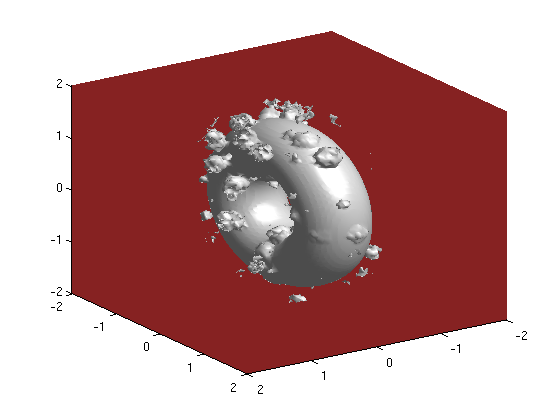
\includegraphics[width=0.5\textwidth]{noise/randNoise/vpmcm/torus/torus100r-0-00}
\caption{Toro al tempo $t=0$, sporcata con rumore random.}
\end{wrapfloat}

In questo test comincia ad emergere in modo più esplicito la
differenza tra i due metodi. Infatti mentre il volume preserving
riesce a ripulire la figura dopo un dato tempo, conservando il volume 
iniziale. L'altro fa collassare il toro ad una circonferenza prima di
pulirlo ed in più per ottenere un risultato osservabile nello stesso
istante temporale in cui il volume preserving completa il denoising,
abbiamo dovuto utilizzare la metà del passo temporale del
volume preserving (vedi \emph{Fig}\ref{fig:cp4-sc2-1-02}). Quindi per
rumori  che hanno  bisogno di un tempo maggiore per essere eliminati,
senza dubbio il volume preserving fornisce dei risultati migliori
rispetto allo schema MCM.

\begin{table}[htb!]
\caption{Tabella per lo schema PVMCM. Evoluzione del Toro nel cubo
  $[-2,2]^3$, sporcato con rumore random.}
\label{tab:cp4-sc2-1-02}
\[
\begin{array}{*{5}{c}l}
    \toprule
    \text{time} &\text{nodi} &\Delta t &\text{iter} &\text{CPUs}&\text{VolErr} \\
    \midrule
     0.03       & 100        & 0.01    & 2          & 38s      &1.7e^{-02}\\
     0.05       &            &         & 4          & 51s      &3.4e^{-02}\\ 
     0.09       &            &         & 8          & 102s     &1.3e^{-01}\\ 
     0.12       &            &         & 10         & 129s     &2,2e^{-01}\\
     \bottomrule
\end{array}
\]
\end{table}

\begin{figure}[htb!]
  \centering
  \subfloat[][\emph{MCM: Toro al tempo} $t=0.05$.]
           {\includegraphics[width=.45\textwidth]{noise/randNoise/mcm/torus/torus100r-2-005}}\quad
  \subfloat[][\emph{MCM: Toro al tempo} $t=0.12$ con $\Delta t=\Delta x/8$.]
           {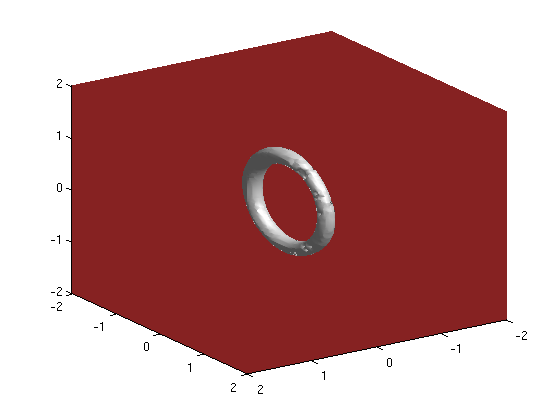
\includegraphics[width=.45\textwidth]{noise/randNoise/mcm/torus/torus100r-4-dt8-012}}\\
  \subfloat[][\emph{PVMCM: Toro al tempo} $t=0.05$.]
           {\includegraphics[width=.45\textwidth]{noise/randNoise/vpmcm/torus/torus100r-2-005}}\quad
  \subfloat[][\emph{PVMCM: Toro al tempo} $t=0.12$.]
           {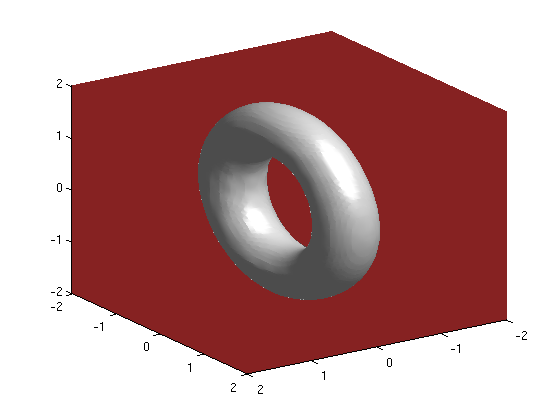
\includegraphics[width=.45\textwidth]{noise/randNoise/vpmcm/torus/torus100r-4-012}}\quad
  \caption{Denoising del manubrio con rumore random.}
  \label{fig:cp4-sc2-1-02}
\end{figure}
\newpage

Concludiamo analizzando il comportamento dei due metodi nel denoising
di una superficie non convessa, sempre sporcata con rumore random.

\begin{wrapfloat}{figure}{l}{0pt}
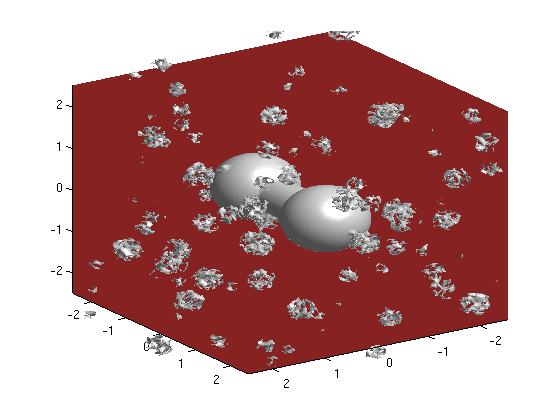
\includegraphics[width=0.5\textwidth]{noise/randNoise/vpmcm/dumbbell/dumb100r-0-00}
\caption{Manubrio al tempo $t=0$, sporcata con rumore random.}
\end{wrapfloat}

Consideriamo il nostro manubrio definito nella sezione
precedente. Lo sporchiamo scegliendo un numero di $300$ sfere con
raggio che varia random  da $0$ a $0.5$ ed addiamo ad aggiungere
 valori random tra $0$ e $0.6$. Come possimao notare nella figura al
 lato c'è molto rumore intorno al manubrio ed un piccola quantità sul
 manubrio stesso. Entrambi i metodi elimano immediatemente il rumore
 che circonda la figura per poi elimira gradualmente il
 restante. Chiaremente, come nel caso de toro, lo schema MCM no
 riesce a terminare il denoising prima che il manubrio si divida in
 due sfere. Mentre con il volume preserving, otteniamo degli ottimi
 risultati (\emph{Fig}\ref{fig:cp4-sc2-1-03}), riuscendo a limitare
 l'errore co volume  iniziale in un ordine di grandezza di $10^{-1}$
 (\emph{Tab}\ref{tab:cp4-sc2-1-03}). 

\begin{table}[htb!]
\caption{Tabella per lo schema PVMCM. Evoluzione del Manubrio nel cubo
  $[-2.5,2.5]^3$, sporcato con rumore random.}
\label{tab:cp4-sc2-1-03}
\[
\begin{array}{*{5}{c}l}
    \toprule
    \text{time} &\text{nodi} &\Delta t &\text{iter} &\text{CPUs}&\text{VolErr} \\
    \midrule
     0.04       & 100        & 0.012   & 3          & 2.7s     &5.8e^{-02}\\
     0.06       &            &         & 5          & 4.7      &1.0e^{-01}\\ 
     0.08       &            &         & 7          & 6.6      &1.1e^{-01}\\ 
     0.09       &            &         & 8          & 7.8s     &1,3e^{-01}\\
     0.14       &            &         & 10         & 10.3s    &1.7e^{-01}\\     
     \bottomrule
\end{array}
\]
\end{table}

\begin{figure}[htb!]
  \centering
  \subfloat[][\emph{MCM: Manubrio al tempo} $t=0.06$.]
           {\includegraphics[width=.45\textwidth]{noise/randNoise/mcm/dumbbell/dumb100r-2-006}}\quad
  \subfloat[][\emph{MCM: Manubrio al tempo} $t=0.14$, con $\Delta
    t=\Delta x /8$.]
           {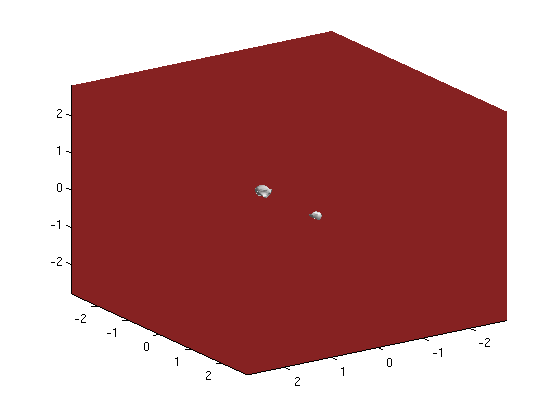
\includegraphics[width=.45\textwidth]{noise/randNoise/mcm/dumbbell/dumb100r-4-014}}\\
  \subfloat[][\emph{PVMCM: Manubrio al tempo} $t=0.06$.]
           {\includegraphics[width=.45\textwidth]{noise/randNoise/vpmcm/dumbbell/dumb100r-2-006}}\quad
  \subfloat[][\emph{PVMCM: Manubrio al tempo} $t=0.14$, con $\Delta
    t=\Delta x /8$.]
           {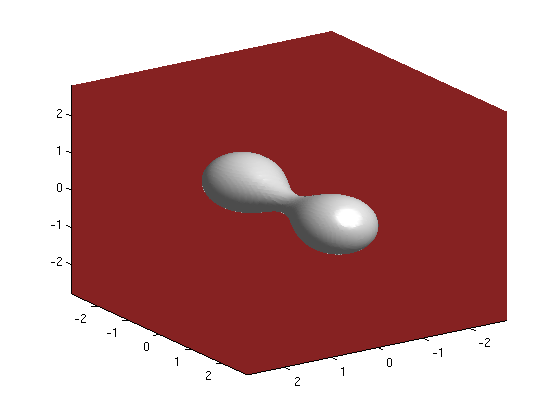
\includegraphics[width=.45\textwidth]{noise/randNoise/vpmcm/dumbbell/dumb100r-4-dt8-014}}\quad
  \caption{Denoising del manubrio con rumore random.}
  \label{fig:cp4-sc2-1-03}
\end{figure}

%%%%%%%%%%%%%%%%%%%%%%%%%%%%%%%%%%%%%%%%%%%%%%%%%%%%%%%%%%%%%%%%%%%%%%%%%%%%%%
%                 Section 4.2.2
%
%%%%%%%%%%%%%%%%%%%%%%%%%%%%%%%%%%%%%%%%%%%%%%%%%%%%%%%%%%%%%%%%%%%%%%%%%%%%%%
\subsection{\emph{Gaussian Noise}}
Nel caso di rumore gaussiano, è stata usata la funzione di MATLAB
\emph{imnoise} sulle superfici standard sfera, toro e manubrio. In
questo caso la differenza tra i due schemi non è molto evidente in
quanto il rumore viene eliminato in tempi brevi, quindi lo schema MCM
non perde troppo volume. Ripotiamo in \emph{Fig}\ref{fig:cp4-sc2-2-01}
i dati iniziali dopo l'aggiunta del rumore e nelle
\emph{Fig}\ref{fig:cp4-sc2-2-02}-\ref{fig:cp4-sc2-2-04} il
denoising. Come possiamo notare nel caso del manubrio, il rumore
gaussiano viene eliminato in tempi brevi, prendendo un  passo
temporale $\Delta t$ più piccolo di $\Delta x$.

\begin{figure}[h!tb]
  \centering
  \subfloat[][\emph{Sfera} al $t=0$.]
           {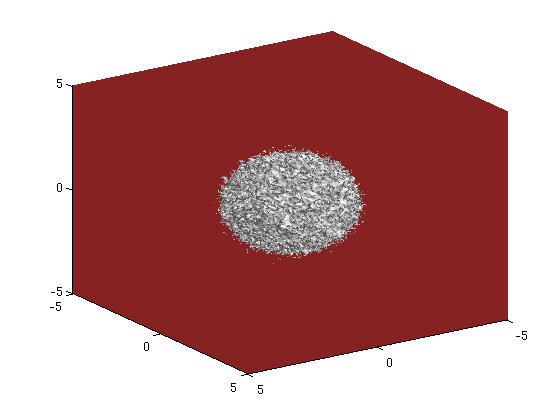
\includegraphics[width=.36\textwidth]{noise/imnoise/mcm/sphere/sphere100i-0-00}}\quad
  \subfloat[][\emph{Toro} al $t=0$.]
           {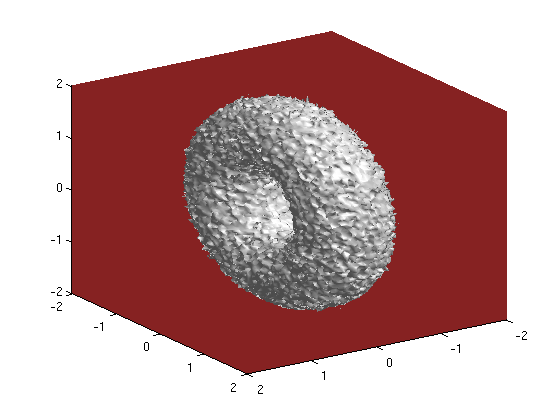
\includegraphics[width=.36\textwidth]{noise/imnoise/mcm/torus/torus100i-0-00}}\\
  \subfloat[][\emph{Manubrio} al $t=0$.]
           {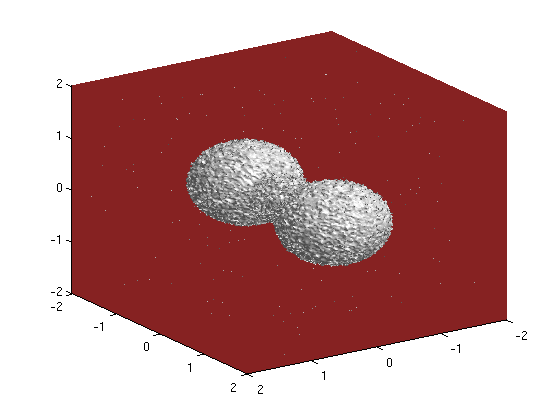
\includegraphics[width=.36\textwidth]{noise/imnoise/mcm/dumbbell/dumb149i-0-00}}\quad
  \caption{Data iniziali genrati dalla funzione \emph{imnoise}.}
  \label{fig:cp4-sc2-2-01}
\end{figure}

\begin{figure}[!htb]
  \centering
  \subfloat[][\emph{MCM: Sfera al tempo} $t=0.1$.]
           {\includegraphics[width=.36\textwidth]{noise/imnoise/mcm/sphere/sphere100i-2-01}}\quad
  \subfloat[][\emph{MCM: Sfera al tempo} $t=0.25$.]
           {\includegraphics[width=.36\textwidth]{noise/imnoise/mcm/sphere/sphere100i-5-025}}\\
  \subfloat[][\emph{PVMCM: Sfera al tempo} $t=0.1$.]
           {\includegraphics[width=.36\textwidth]{noise/imnoise/vpmcm/sphere/sphere100i-2-01}}\quad
  \subfloat[][\emph{PVMCM: Sfera al tempo} $t=0.25$.]
           {\includegraphics[width=.36\textwidth]{noise/imnoise/vpmcm/sphere/sphere100i-5-025}}\quad
  \caption{Denoising della Sfera con rumore gaussiano.}
  \label{fig:cp4-sc2-2-02}
\end{figure}


\begin{figure}[h!tb]
  \centering
  \subfloat[][\emph{MCM: Toro al tempo} $t=0.05$.]
           {\includegraphics[width=.36\textwidth]{noise/imnoise/mcm/torus/torus100i-2-005}}\quad
  \subfloat[][\emph{MCM: Toro al tempo} $t=0.12$.]
           {\includegraphics[width=.36\textwidth]{noise/imnoise/mcm/torus/torus100i-5-012}}\\
  \subfloat[][\emph{PVMCM: Toro al tempo} $t=0.05$.]
           {\includegraphics[width=.36\textwidth]{noise/imnoise/vpmcm/torus/torus100i-2-005}}\quad
  \subfloat[][\emph{PVMCM: Toro al tempo} $t=0.12$.]
           {\includegraphics[width=.36\textwidth]{noise/imnoise/vpmcm/torus/torus100i-5-012}}\quad
  \caption{Denoising del toro con rumore gaussiano.}
  \label{fig:cp4-sc2-2-03}
\end{figure}

\begin{figure}[htb!]
  \centering
  \subfloat[][\emph{MCM: Manubrio al tempo} $t=0.01$, con $\Delta
   t=\Delta x /4$.]
           {\includegraphics[width=.36\textwidth]{noise/imnoise/mcm/dumbbell/dumb149i-2-dt4-001}}\quad
  \subfloat[][\emph{MCM: Manubrio al tempo} $t=0.01$, con $\Delta t=\Delta x /32$.]
           {\includegraphics[width=.36\textwidth]{noise/imnoise/mcm/dumbbell/dumb149i-4-dt32-001}}\\
  \subfloat[][\emph{PVMCM: Manubrio al tempo} $t=0.01$, con $\Delta
    t=\Delta x /8$.]
           {\includegraphics[width=.36\textwidth]{noise/imnoise/vpmcm/dumbbell/dumb149i-2-dt4-001}}\quad
  \subfloat[][\emph{PVMCM: Manubrio al tempo} $t=0.01$, con $\Delta
    t=\Delta x /32$.]
           {\includegraphics[width=.36\textwidth]{noise/imnoise/vpmcm/dumbbell/dumb149i-4-dt32-001}}\quad
  \caption{Denoising del manubrio con rumore gaussiano.}
  \label{fig:cp4-sc2-2-04}
\end{figure}

%%%%%%%%%%%%%%%%%%%%%%%%%%%%%%%%%%%%%%%%%%%%%%%%%%%%%%%%%%%%%%%%%%%%%%%%%%%%%%
%                 Section 4.3
%
%%%%%%%%%%%%%%%%%%%%%%%%%%%%%%%%%%%%%%%%%%%%%%%%%%%%%%%%%%%%%%%%%%%%%%%%%%%%%%
\section{Immagini reali. Il \emph{Gargolye}}
In questa sezione andremo ad testare entrambi i metodi su di un'immagine 3D reale.  

\begin{wrapfloat}{figure}{l}{0pt}
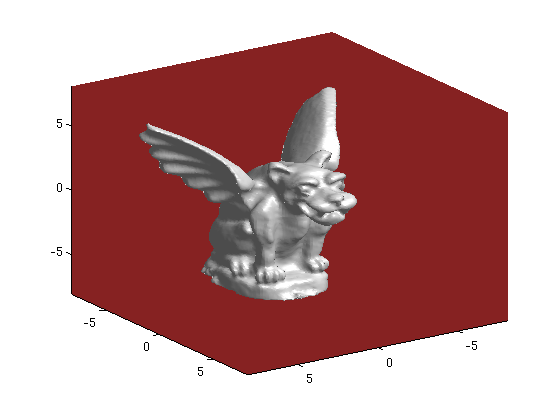
\includegraphics[width=0.5\textwidth]{smooth/vpmcm/gargolye/garg149-0-00}
\caption{Gargolye al tempo $t=0$ ed al livello zero, ottenuta da un scanner 3D.}
\label{fig:cp4-sc3-01}
\end{wrapfloat}

L'immagine scelta rappresenta un \emph{gargolye} e ci è stata fornita
dal laboratorio della focoltà di matematica dell'universita di
Bologna. Il gargolye è stato importato grazie all'utilizzo di uno
scanner 3D, che ci ha restituito i valori della funzione level-set che
rappresenta tale superficie (\emph{Fig}\ref{fig:cp4-sc3-01}).  Chiaramente tale funzione non presenta le stesse regolarità di quelle utilizzate nei test
precedenti, per cui dopo un tot di iterazioni l'immagine comincia un
processo di erosione (\emph{Fig}\ref{fig:cp4-sc3-03}). Iniziamo col
far evolvere ll gargolye senza l'aggiunta di rumore. Premettiamo che i
valori del gargolye ci sono stati forniti nell'intervallo $[1,149]$ con
$\Delta x=1$, ora in quanto utilizziamo dei metodi di approssimazione
del volume che sono dell'ordine di $\Delta x$, abbiamo deciso di
riscalare il tutto nell'intervallo $[-8,8]$, al fine di lavorare con
un passo spaziale più piccolo. Il comportamento differente dei due metodi,
data l'impossibilità, come anticipato poc'ansi, di effettuare troppe
iterazioni ed di aumentare i nodi della griglia, non è immediatamenti
evidente nelle immagini (\emph{Fig}\ref{fig:cp4-sc3-02}), ma si può
dedurre dall'analisi delle
\emph{Tab}\ref{tab:cp4-sc3-01}-\ref{tab:cp4-sc3-02}. In queste è stato
riportato  l'errore in norma tra il volume iniziale e quello finale,
anche se sembra alto tuttavia è da notare che il volume del gargolye è
circa $170$ quindi l'errore relativo del metodo volume preserving
sarebbe dell'ordine di $10^{-2}$, mentre del MCM dell'ordine di
$10^{-1}$. Osserviamo inoltre (vedi \emph{Tab}\ref{tab:cp4-sc3-02})
che dimezzando il passo temporale nello schema volume preserving
l'errore migliora, tuttavia questo comporta anche l'aumento delle
iterazioni temporali generando risultati come in \emph{Fig}\ref{fig:cp4-sc3-03}.

\begin{table}[htb!]
\caption{Tabella per lo schema MCM. Evoluzione del Gargolye nel cubo
  $[-8,8]^3$.}
\label{tab:cp4-sc3-01}
\[
\begin{array}{*{5}{c}l}
    \toprule
    \text{time} &\text{nodi} &\Delta t &\text{iter} &\text{CPUs}&\text{VolErr} \\
    \midrule
     0.01       & 149        & 0.01    & 1          & 0.7s     &13\\
     0.05       &            & 0.02    & 2          & 1.8s     &20.5\\ 
     0.15       &            & 0.1     & 2          & 1.8s     &24\\ 
     0.25       &            &         & 3          & 3.4s     &32.1\\
     0.14       &            & 0.05    & 5          & 7.7s    &40.1\\     
     \bottomrule
\end{array}
\]
\end{table}

\begin{table}[htb!]
\caption{Tabella per lo schema PVMCM. Evoluzione del Gargolye nel cubo
  $[-8,8]^3$.}
\label{tab:cp4-sc3-02}
\[
\begin{array}{*{5}{c}l}
    \toprule
    \text{time} &\text{nodi} &\Delta t &\text{iter} &\text{CPUs}&\text{VolErr} \\
    \midrule
     0.01       & 149        & 0.01    & 1          & 1.5s     &1.5\\
     0.05       &            & 0.02    & 2          & 3.6s     &2.1\\ 
     0.15       &            & 0.1     & 2          & 3.6s     &12.6\\ 
     0.25       &            &         & 3          & 7.0s     &19.1\\
     0.14       &            & 0.05    & 5          & 16.0s    &13.2\\     
     \bottomrule
\end{array}
\]
\end{table}

\begin{figure}[h!tb]
  \centering
  \subfloat[][\emph{MCM: Gargolye al tempo} $t=0.01$, con $\Delta
    t=\Delta x/8$.]
           {\includegraphics[width=.45\textwidth]{smooth/mcm/gargolye/garg149-1-dt8-001}}\quad
  \subfloat[][\emph{MCM: Gargolye al tempo} $t=0.15$, con $\Delta
     t=\Delta x$.]
           {\includegraphics[width=.45\textwidth]{smooth/mcm/gargolye/garg149-3-dt-015}}\\
  \subfloat[][\emph{PVMCM: Gargolye al tempo} $t=0.01$ con $\Delta
    t=\Delta x/8$.]
           {\includegraphics[width=.45\textwidth]{smooth/vpmcm/gargolye/garg149-1-dt8-001}}\quad
  \subfloat[][\emph{PVMCM: Gargolye al tempo} $t=0.15$ con $\Delta
    t=\Delta x$.]
           {\includegraphics[width=.45\textwidth]{smooth/vpmcm/gargolye/garg149-3-dt-015}}\quad
  \caption{Evoluzione del Gargolye.}
  \label{fig:cp4-sc3-02}
\end{figure}

\begin{figure}[h!tb]
  \centering
  \subfloat[][\emph{MCM: Gargolye al tempo} $t=0.25$, con $\Delta
      t=\Delta x/2$.]
           {\includegraphics[width=.35\textwidth]{smooth/mcm/gargolye/garg149-4-dt2-025}}\quad
  \subfloat[][\emph{PVMCM: Gargolye al tempo} $t=0.25$ con $\Delta
    t=\Delta x/2$.]
           {\includegraphics[width=.35\textwidth]{smooth/vpmcm/gargolye/garg149-5-dt2-025}}\quad
  \caption{Erosione del Gargolye.}
  \label{fig:cp4-sc3-03}
\end{figure}

Andiamo ora ad aggiungere il rumore all'immagine iniziale e
effettuiamo il denoising. Inizieremo con il rumore random. In
\emph{Fig}\ref{fig:cp4-sc3-04-a} abbiamo aggiunto rumore inserendo
$500$ sfere con raggio piccolo, in un range da $0$ a $0.05$ e facendo
variare i valori del rumore tra $0$ e $0.6$. Mentre in
\emph{Fig}\ref{fig:cp4-sc3-04-b} abbiamo preso una sola sfera con
raggio grande e valori del rumore piccoli, in modo tale che questo si trovi maggiormente sulla superfice del gargoolye. 

\begin{figure}[h!tb]
  \centering
  \subfloat[][\emph{Gargolye al tempo} $t=0.0$,rumore random con $500$
    sfere con raggi tra $0$ e $0.05$ e rumore tra $0$ e $0.6$.\label{fig:cp4-sc3-04-a}]
           {\includegraphics[width=.45\textwidth]{noise/randNoise/mcm/gargolye/garg149r4-0-00}}\quad
  \subfloat[][\emph{Gargolye al tempo} $t=0.0$, rumore random con $1$
    sfera con raggio tra $0$ e $100$ e rumore tra $0$ e
    $0.0001$. \label{fig:cp4-sc3-04-b}]
           {\includegraphics[width=.45\textwidth]{noise/randNoise/vpmcm/gargolye/garg149r3-0-00}}\quad
  \caption{Gargolye con rumore random.}
  \label{fig:cp4-sc3-04}
\end{figure}

Entrambi i metodi puliscono l'immagine in modo accettabbile e sembra
che si comportino in modo del tutto simile (vedi
\emph{Fig}\ref{fig:cp4-sc3-05}-\ref{fig:cp4-sc3-06}). Per osservare le
differenze nella conservazione del volume, dobbiamo analizzare le tabelle
\emph{Tab}\ref{tab:cp4-sc3-02}-\ref{tab:cp4-sc3-02} precedenti, in
quanto gli errori sono simili al caso senza rumore. Questo è dovuto al
fatto che abbiamo preso dei rumori random piccoli, data
l'impossibilità di fare troppo iterazioni per pulire
l'immagine. Stesse considerazioni valgono anche nel caso di rumore
gaussiano dove abbiamo utilizzato un valore di media pari a zero e
varianza pari a $10^{-8}$. In queste condizioni siamo riusciti a
ricreare un rumore che entrambi i metodi eliminano in tempi brevi
(\emph{Fig}\ref{fig:cp4-sc3-07}), prima di trovarci nella situazione ripotata in
\emph{Fig}\ref{fig:cp4-sc3-03}. 

\begin{figure}[h!tb]
  \centering
  \subfloat[][\emph{MCM: Gargolye al tempo} $t=0.01$, con $\Delta t =
    \Delta x/8$.]
           {\includegraphics[width=.45\textwidth]{noise/randNoise/mcm/gargolye/garg149r4-1-dt8-001}}\quad
  \subfloat[][\emph{MCM: Gargolye al tempo} $t=0.15$, con $\Delta t =
    \Delta x$]
           {\includegraphics[width=.45\textwidth]{noise/randNoise/mcm/gargolye/garg149r4-4-dt-015}}\\
  \subfloat[][\emph{VPMCM: Gargolye al tempo} $t=0.01$, con $\Delta t =
    \Delta x/8$.]
           {\includegraphics[width=.45\textwidth]{noise/randNoise/vpmcm/gargolye/garg149r4-1-dt8-001}}\quad
  \subfloat[][\emph{VPMCM: Gargolye al tempo} $t=0.15$, con $\Delta t =
    \Delta x$]
           {\includegraphics[width=.45\textwidth]{noise/randNoise/vpmcm/gargolye/garg149r4-4-dt-015}}
  \caption{Evoluzione del Gargolye in \emph{Fig}\ref{fig:cp4-sc3-04-a}.}
  \label{fig:cp4-sc3-05}
\end{figure} 

\begin{figure}[h!tb]
  \centering
  \subfloat[][\emph{MCM: Gargolye al tempo} $t=0.01$, con $\Delta t =
    \Delta x/8$.]
           {\includegraphics[width=.45\textwidth]{noise/randNoise/mcm/gargolye/garg149r3-1-dt8-001}}\quad
  \subfloat[][\emph{MCM: Gargolye al tempo} $t=0.03$, con $\Delta t =
    \Delta x/8$]
           {\includegraphics[width=.45\textwidth]{noise/randNoise/mcm/gargolye/garg149r3-2-dt8-003}}\\
  \subfloat[][\emph{VPMCM: Gargolye al tempo} $t=0.01$, con $\Delta t =
     \Delta x/8$.]
           {\includegraphics[width=.45\textwidth]{noise/randNoise/vpmcm/gargolye/garg149r3-1-dt8-001}}\quad
  \subfloat[][\emph{VPMCM: Gargolye al tempo} $t=0.03$, con $\Delta t =
    \Delta x/8$]
           {\includegraphics[width=.45\textwidth]{noise/randNoise/vpmcm/gargolye/garg149r3-2-dt8-003}}
  \caption{Evoluzione del Gargolye in \emph{Fig}\ref{fig:cp4-sc3-04-b}.}
  \label{fig:cp4-sc3-06}
\end{figure}

\begin{figure}[h!tb]
  \centering
  \subfloat[][\emph{Gargolye al tempo} $t=0.0$, con rumore gaussiano]
           {\includegraphics[width=.45\textwidth]{noise/imnoise/mcm/gargolye/garg149i-0-00}}\\
  \subfloat[][\emph{MCM: Gargolye al tempo} $t=0.01$, con $\Delta t =
    \Delta x/8$.]
           {\includegraphics[width=.45\textwidth]{noise/imnoise/mcm/gargolye/garg149i-1-dt8-001}}\quad
  \subfloat[][\emph{MCM: Gargolye al tempo} $t=0.15$, con $\Delta t =
    \Delta x$]
           {\includegraphics[width=.45\textwidth]{noise/imnoise/mcm/gargolye/garg149i-3-dt-015}}\\
  \subfloat[][\emph{VPMCM: Gargolye al tempo} $t=0.01$, con $\Delta t =
     \Delta x/8$.]
           {\includegraphics[width=.45\textwidth]{noise/imnoise/vpmcm/gargolye/garg149i-1-dt8-001}}\quad
  \subfloat[][\emph{VPMCM: Gargolye al tempo} $t=0.15$, con $\Delta t =
    \Delta x$]
           {\includegraphics[width=.45\textwidth]{noise/imnoise/vpmcm/gargolye/garg149i-3-dt-015}}
  \caption{Evoluzione del Gargolye con rumore gaussiano.}
  \label{fig:cp4-sc3-07}
\end{figure}  

